%%%%%%%%%%%%%%%%%%%%%%%%%%%%%%%%%%%%%%%%%%%%%%%%%%%%%%%%%%%%%%%%%%%%%%%%%%%%%%%%
\section{(ii) Urban Performance Inference with Telecom Data}

 {
  Following the work done using CDR data\footnote{see Section \eqref{sec:andorra-data-observatory}, and references \cite{leng2016analysis, grignard2017agent}}, the Andorran Government offered several new data pipelines containing high resolution location data. Radio Network Controller (RNC), a statewide location data source became available for multiple periods between 2015-2021. Using RNC, two statistical models were developed to explore the relationship between the physical features of Andorran cities and the discrete behavior of its residents and visitors. These models highlighted various dependencies and detractions between certain urban-design settings, and human behavioral patterns. This study suggests a method of statistical analysis to evaluate the performance of public spaces, as a proxy of the prevalence of certain behaviors to occur.
 }

\subsection{Introduction}

{
    Vibrant public spaces that attract dense and diverse populations, are an integral part of any successful urban district \cite{krier1979urban, banerjee2011companion, gehl2013study}. Nevertheless, accurate correlation between public spaces and human activity is hard to measure and analyze \cite{gehl2013study, Calabrese2014}. In recent decades, data-driven methods for the analysis of urban places, became possible using Location-Based Services and new statistical processing techniques \cite{Hillier1993}.
    This work marries a high-resolution location dataset, and a set of urban properties, to infer the relationships between human behavior and spatial arrangement of public spaces. The rest of this section details the site and data used in this work.

    \subsubsection{Study Area}
    {
        The city center of Andorra is located in a steep Valley made by the Valira river (100m - 600m width). This topography formed an organically shaped urban-center that merges with its natural surroundings. Andorra has no airport or train service, so that the majority of nearly 8 million visitors per year arrive by motorized vehicles from either Spain or France \cite{CIA}. Both Andorra La-Vella and Les Escaldes municipalities were considered in this study.
    }

    \subsubsection{Data}
    {
        Andorra Telecom (AT), the sole telecoms service in Andorra, provided the data for this study. Having a singular country-wide telecom provider, differentiates this dataset from those acquired in other cities, where a fragmented market usually holds multiple cellular providers \cite{louail2014mobile}. The third generation (3G) network operated by AT is a Universal Mobile Telecommunications System (UMTS) network and the governing element of the UMTS network is the Radio Network Controller (RNC) \cite{ETSI}. One function of the RNC is to keep track of the locations of devices as they move around the coverage area, without the need for an active device usage. Each time a connected device interacts with the network (through call, text or cellular data), moves from one cell tower to another, or goes unobserved for more than 90 minutes, an observation is recorded. Each observation includes a unique id for the subscriber, a timestamp, the device coordinates at the time of the update, and the home network of the subscriber. The coordinates are given in the standard WGS84 system, estimated by AT to be within 25-100m in urban areas, significantly more precise than Call Detail Records (CDR) \cite{gonzalez2008understanding, Deville2014, blondel2015survey}. AT utilizes enhanced triangulation using the angle, time and RSS received by the device from different base-stations, as well as error mitigation using a proprietary algorithm. For the purpose of the study, data from Saturdays in September 2016 were used. Only Saturdays were considered, in order to focus on social activity rather than work activity, and the two days chosen were ones without any large cultural events which could create anomalies.
    }
}

\subsection{Methodology}
{
    In order to model the relationship between human activity and urban-design, two pre-processing steps were taken: (i) The aggregation of human behavior into clusters, and (ii) the agglomeration of urban features, POIs, and amenities, as explanatory variables. This Section describes these pre-processing steps.
}

\subsubsection{Stay-events and Activity Clusters}
{

    \begin{figure}[!h]
        \begin{center}
            \includegraphics[width=1\textwidth]{chapters/insight/revurb/figures/revurb_data.png}
        \end{center}
        \caption{Stays and Cluster. (left) Stay events analysis over 24hrs duration and the DBSCAN method which extracts clusters. (right) clusters culling based on `persistance', which is the duration a moving cluster sustain throughout the day.}
        \label{fig:revurb_data}
    \end{figure}

    In this work, urban behavior is evaluated through the formation of dense clusters of non-transient activity. These clusters are considered to be important as they allow to identify not only those places in which individuals spend time, but the places where diverse groups of people congregate together, creating the potential for social interaction. The identification of activity clusters is carried out by a 2-step procedure: (i) finding stay-points and (ii) clustering those stay-points with certain parameters. The overall process is illustrated in Figure \eqref{fig:revurb_clusters}.
    \newline
    \textbf{Stay-events:} The purpose of the first step is to eliminate `roaming' observations (i.e., where a person is only passing through an area), and retain only events where a person has intentionally stayed in a particular vicinity for a certain amount of time. A stay-point is defined as a group of observations of a person's location, whereby no point is greater than 200m from any other point and the time elapsed is at least 20 minutes \cite{li2008mining}. The maximum distance and minimum time parameters were considered appropriate as they would filter out common roaming events, while preserving activities for which this particular location has been chosen.

    \begin{figure}[!h]
        \begin{center}
            \includegraphics[width=0.75\textwidth]{chapters/insight/revurb/figures/revurb_clusters.png}
        \end{center}
        \caption{Clustering stay-points as `Moving Clusters'. Each potential cluster was deemed relevant considering its longevity, density, and diversity. The map show clusters formed near the city-center.}
        \label{fig:revurb_clusters}
    \end{figure}

    \textbf{Clusters:} Following the identification of individual stay-points, a density based clustering algorithm was used in each 10-minute time period to find locations where groups of individuals congregate together. Such algorithms agglomerate some points to clusters while leaving other points un-clustered, so that the density of stay points within the clusters is considerably higher than the density of points outside of the clusters. The clustering algorithm is Density-Based Spatial Clustering of Applications with Noise (DBSCAN) \cite{ester1996density}, which is capable of efficiently finding clusters of arbitrary shape, size and quantity\footnote{DBSCAN is based on the notion that the density of a point in a dataset is a function of its spatial-temporal proximity to other points in the dataset, hence it overcome clustering issues that appear in other methods, such as K-means or PCA \cite{ester1996density}.}. In relating the clusters to urban features, each cluster was represented by its centroid; Since individual RNC observations had a standard error of ~50m, the coverage region of the cluster could not be known with enough precision. However, the standard error of the cluster centroid decreases with the number of observations, making this estimate much more reliable.
    \newline
    \textbf{Findings:} Some insights could already be gained from observation of the produced clusters, prior to any model fitting: Clusters tended to form along the main river passing through the city, as well as near commercial centers, including `Leclerc' supermarket, and cultural museums, such as Natural History Museum and Carmen Thyssen Museum. On the contrary, clusters were less likely to form around big urban green spaces and sparsely built environments. These insights are expected, given the tendency of human activity to form along geographical features, leisure places, and amenities. Nevertheless, the goal of this study was to provide a high-resolution explanatory model that can show which urban features and their agglomeration are highly correlated with clusters of activity.
}

\subsubsection{Identifying Urban Features} \label{subsec:urbFeat}

{
    \begin{figure}[!h]
        \begin{center}
            \includegraphics[width=0.75\textwidth]{chapters/insight/revurb/figures/revurb_features.png}
        \end{center}
        \caption{Urban features, temporal data and the city. Isometric view of the different datasets and urban features used in this study. Purple layers represent static data, and pink layers represent temporal and dynamic observations.}
        \label{fig:revurb_layers}
    \end{figure}

    In order to relate the activity clusters to spatial features, a set of candidate features was proposed. This list considered core elements of the public realm, such as transportation networks, landscape elements, or commercial buildings, which might be more likely to influence the creation of activity clusters. These correspond to classic urban theories, such as the five elements of mental maps \cite{lynch1960image}, the pattern languages \cite{alexander1977pattern}, as well as contemporary urban-design evaluation frameworks \cite{hassan2014evaluation}. Included in the feature set were locations of amenities from the Google Places API, as well as bus stops, GIS shape files of buildings, roads, green spaces, water features and car parks from OpenStreetMap \cite{haklay2008openstreetmap}. Figure \eqref{fig:revurb_layers} shows the various stages of processing the RNC data along with the categories of urban features considered in the model fitting. Appendix Table \eqref{tab:andorra_model_features} lists the features considered in the model fitting.
}

\subsubsection{Subdivision of Study Area}
{
    In this study, a single measure of behavioral pattern (clusters) and the associated set of urban features (form, function, or morphology) would constitute a single observation. However, as in many other instances of spatial analysis, the observed data is based on events occurring in continuous space and time, and therefore do not naturally form such a structure. For this reason, it is common to subdivide the study area into spatial polygons with defined boundaries; These polygons are then used as bins to aggregate the observed data into discrete observations \cite{bivand2008applied}.
    \newline
    In the case of Andorra's physical formation, no obvious morphological tessellation of the study region was apparent. The natural landscape formed by the Pyrenees mountains forced an organic urban form to evolve, making urban blocks or road network grid unconstrained enough for analysis. As shown in the upper part of Figure \eqref{fig:revurb_layers}, the city center of Andorra was instead divided into a regularly spaced grid of $50mx50m$ cells. The size of the cells was chosen in order to be at the scale of the urban features, as well as within the bounds of the telecom data accuracy threshold\footnote{At an early stage of this work, a 25sqm grid was attempted but resulted in a lower model fit.}. All of the behavioral and urban feature metrics were computed for every grid cell in the study region, 962 in total.
}

\subsection{Models}
{

    The location data was preprocessed through DBSCAN, an unsupervised clustering algorithm, in order to groups together activities across time and space. Following the clustering, two methods were developed to examine the relationship between human behavior, and the usage patterns of urban feature:
    \newline
    (i) The first uses two supervised learning algorithms, \textbf{Multivariate Linear regression} (MLR and Lasso MLR), which were fit to the clusters in order to asses total clustering population, normalized clustering time and clustering diversity, and suggest which amenities are more representative for the creation of these clusters.
    \newline
    (ii) The second model is based on \textbf{Inhomogeneous Poisson Process (IPP)}, a density based clustering algorithm, where the density of a process varies in space in association with the urban features. The IPP intensity was found to be positively associated with amenities such as shopping and entertainment, the availability of parking and bus stops and the presence of natural water features. The intensity was negatively associated with the distance from the city centre and streets and with presence of hotels.
    \newline
    Both models are detailed in the following sections.
}

\subsection{(i) MLR and Lasso Regression}
{
    The first modeling method uses two flavors of regression models: Multivariate Linear Regression (MLR) and Lasso Multivariate Linear Regression (Lasso). Results from both methods are included in this study as MLR provides intuitive results which include p-values, whereas lasso MLR provides additional validation to the results \cite{neter1996applied}\footnote{See Appendix Section \eqref{appendix:mlr_and_lasso_mlr} for more on the differences and advantages of using both methods}.

    \subsubsection{MLR Model Training}\label{mlr_model_training}
    {
        Three variants of this model were fit to the data: (i) total clustering population, (ii) normalized clustering time, and (iii) clustering diversity. In order to identify the best fitting model, a forward stepwise search was carried out from the null model to a model including all variables. At each step, a single variable was chosen to be added to the model based on how much it would improve the Akaike Information Criterion (AIC) of the model. If there were no variables remaining whose addition to the model would include the AIC, the stepwise search concluded with the current model.
    }

    \subsubsection{MLR Results}
    {
        Over a period of 16 days (between Sept. 15 - 30, 2016) 2,422,065 stay-points and 10,908 moving clusters were identified. The results of the model fitting process are presented in table \eqref{tab:mlr-results}:
    }

    \begin{table}
        \caption{Model results. (N: Number, B: Binary, I: Index, MSE: Mean squared error, CV: Cross validation, SE: Standard Error)}
        \begin{center}
            \begin{tabular}{l|llcl}
                \multirow{2}{*}{\textbf{\begin{tabular}[c]{@{}l@{}}Variable:\\ Services {[}N{]}\end{tabular}}} & \multicolumn{3}{l}{\textbf{Multivariate Regression}} & \textbf{Lasso}                                                  \\
                                                                                                               & \textbf{Coefficient}                                 & \textbf{p-value} & \textbf{Significance} & \textbf{Coefficient} \\

                \noalign{\hrule height 0.25pt}
                Size                                                                                           & 0.15                                                 & 4.84E-11         & ***                   & 0.12                 \\
                Persistence                                                                                    & 0.31                                                 & 6.40E-10         & ***                   & 0.27                 \\
                Diversity                                                                                      & 0.28                                                 & 0.00678          & **                    & 0.22                 \\
            \end{tabular}
        \end{center}
        \label{tab:mlr-results}
    \end{table}

}


\subsection{(ii) Point Process Model} \label{sec:ppm}

{
    The second modeling method is a Point Process Model. This approach is a better fit for events distributed over time and space, such as the clustering of time-series stay-points and urban features. A point process is a stochastic mechanism that generates a countable set of events inside a region of space \cite{diggle2013statistical}. Occasionally, a point process may exhibit Complete Spatial Randomness (CSR). In such cases the process may be modelled as a Homogeneous Poisson Process \cite{baddeley2008analysing}. This model describes the expected number of points, \textit{P}, found in any arbitrary window \textit{B} as
    $
        \mathbb{E}[count(P \quad in \quad B)] = \lambda \times area(B)\inlineeqno{(1)}
    $
    where $\lambda$ is the intensity of the process. Homogeneous Poisson Processes are rarely used in practical applications, as most point patterns have intensity which varies in space, often in association with one or more covariates. In this case, the process may be modelled as an Inhomogeneous Poisson Process (IPP). This model describes the expected number of points found in any arbitrary window as
    $
        \mathbb{E}[count(P \quad in \quad B)] = \int_{B}\lambda(u)du \inlineeqno{(2)}
    $
    where the intensity $\lambda$ is a function of the covariates $x_1(u)$ to $x_n(u)$.
    $
        \lambda(x)=\exp(\beta_0+\beta_1x_1(u)+\beta_2x_2(u)+...)\inlineeqno{(3)}
    $
    All clusters found over the data duration were aggregated to form a 2-dimensional point-pattern in continuous space throughout the study region. The Inhomogeneous Poisson Process (IPP) is used to model the occurrence of activity clusters as a function of the set of urban features described above.
    \newline
    In order to include urban features as covariates in the IPP model, they must each be represented as a 2 dimensional image. For the point features, which included locations of amenities and bus-stops, kernel-smoothed densities were used. The kernels were all Gaussian with a standard-deviation of 20m. For the polygon features such as buildings, binary masks were used. The IPP model can be fitted to the data by maximizing the log-likelihood function using the Berman-Turner algorithm \cite{berman1992approximating}.
    The fitting process was carried out using the \textit{R} computing software using the \textit{spatstat} package \cite{baddeley2005spatstat}. Each of the features described in section \eqref{subsec:urbFeat} was considered for inclusion in the model. As with the MLR model, in order to prevent model over-fitting, a forward step-wise selection procedure was used \cite{friedman2001elements}. An advantage of this method is that a fitted IPP model can be used to simulate new sets of cluster locations for any other similar region, where the urban features can be similarly measured.
}

\subsection{Results and Discussion}
{


    \begin{figure}[!h]
        \centering
        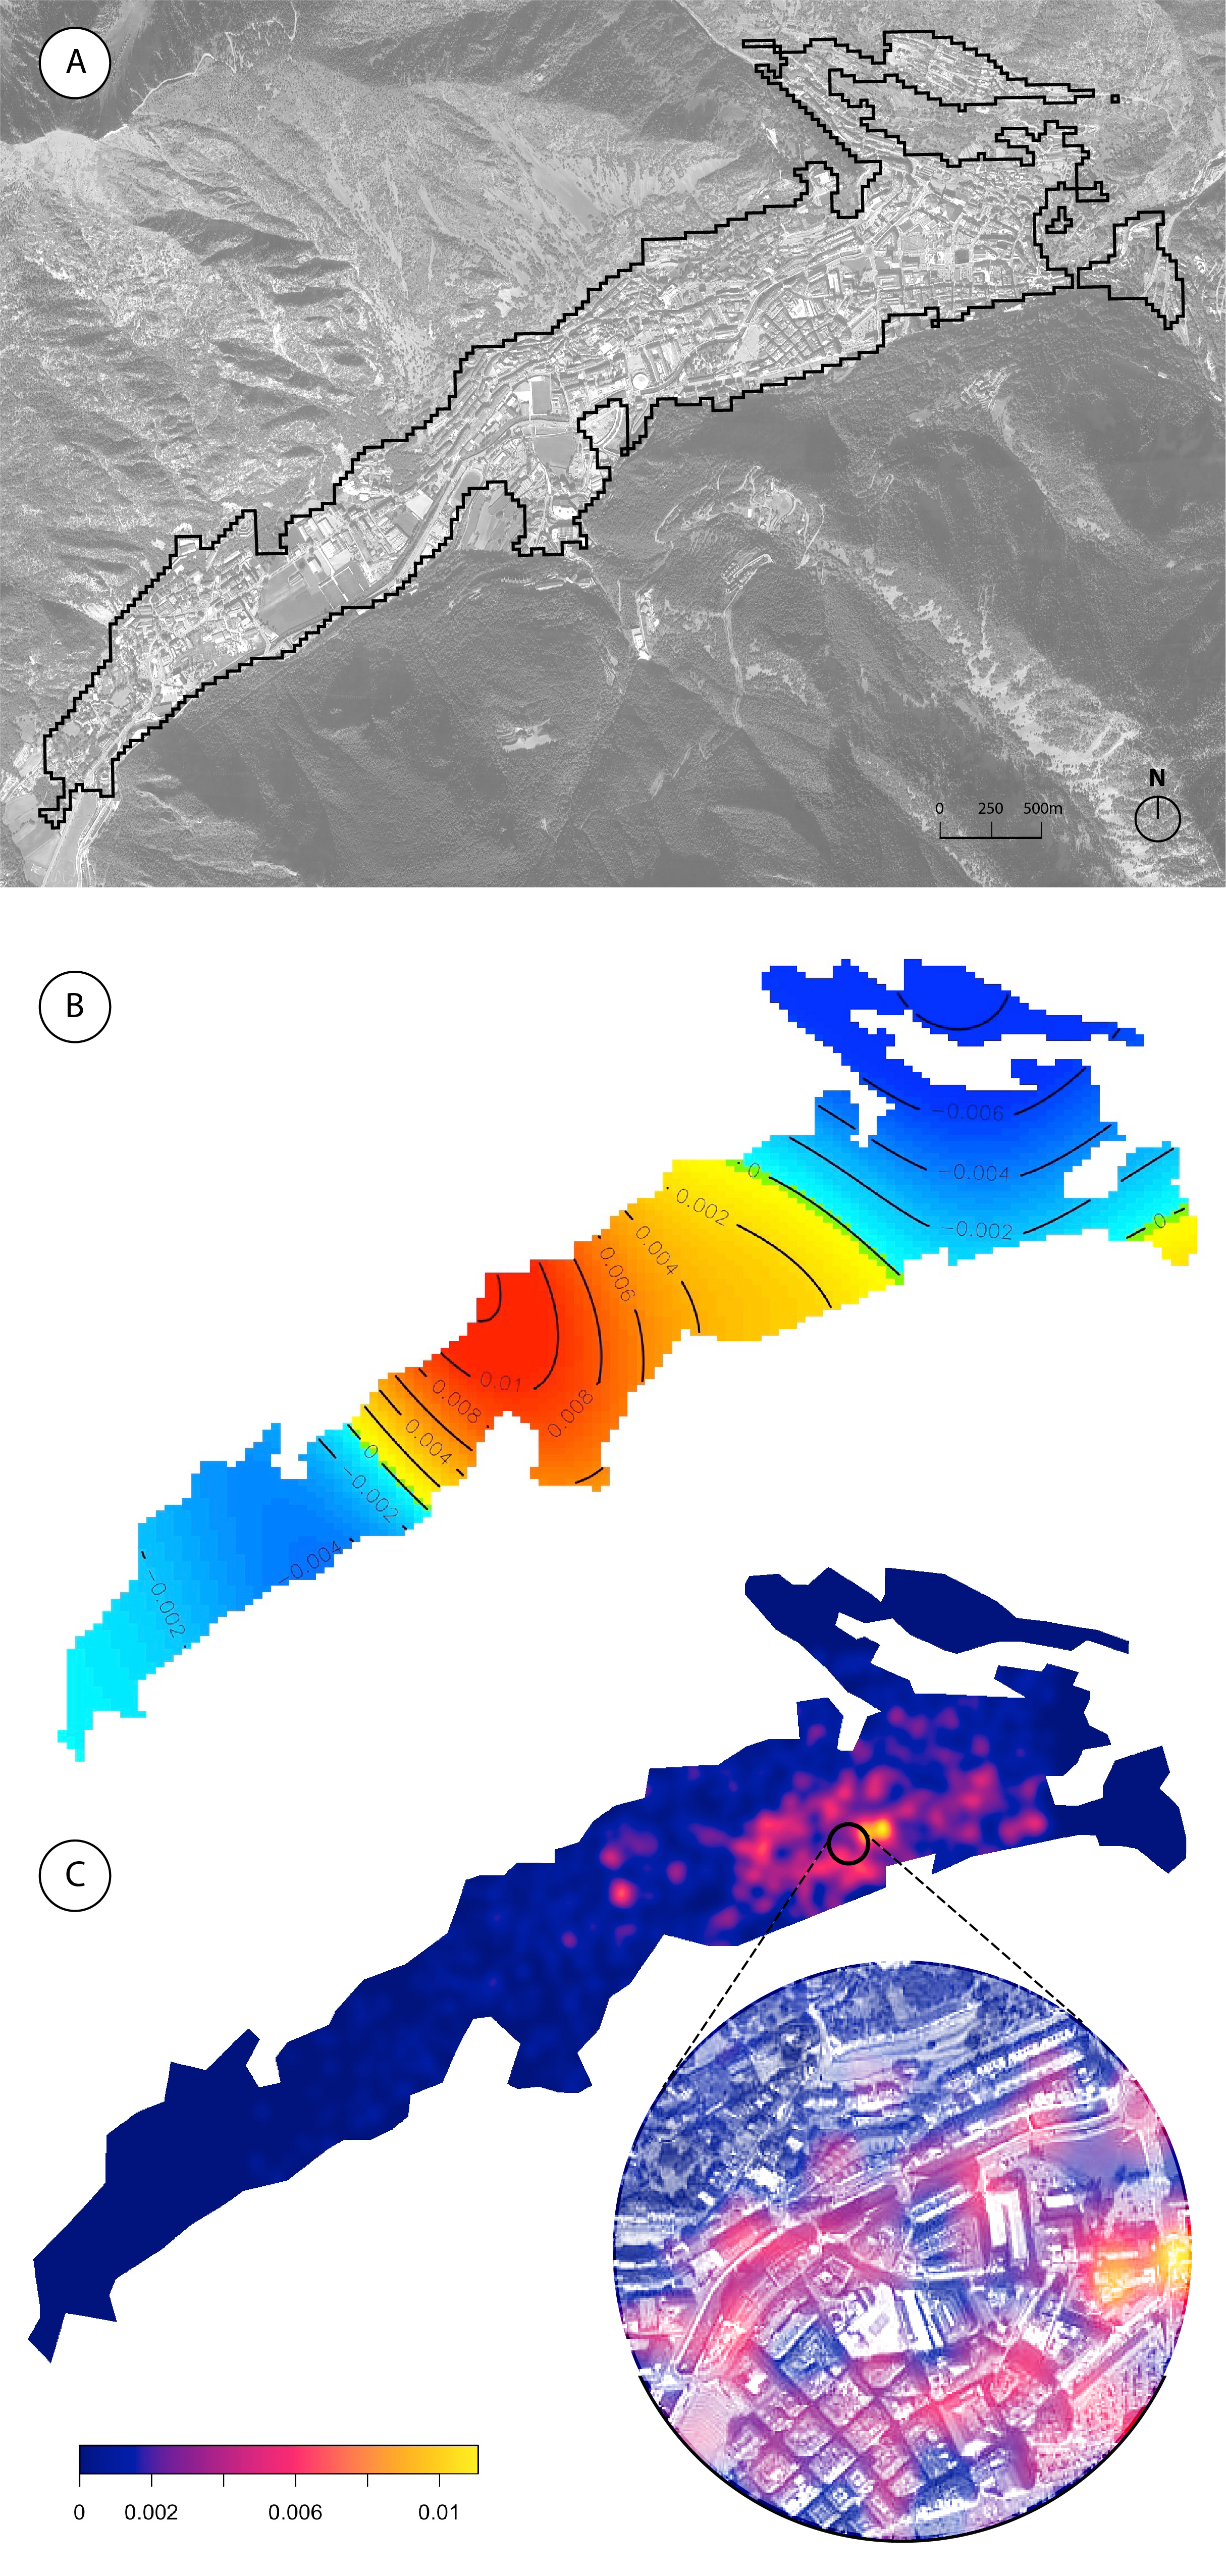
\includegraphics[width=0.5\textwidth]{chapters/insight/revurb/figures/revurb_ppm.jpg}
        \caption{Model area and densities. (a) Study region, (b) Contour plot of Pearson residuals from fitted model, (c) Smoothed density of points simulated from Inhomogeneous Poison Process model}
        \label{fig:ppm_res}
    \end{figure}

    The step-wise selection procedure outlined in Section \eqref{sec:ppm} resulted in a model which included 14 of the 16 urban features considered. The only variables excluded due to their failure to improve the AIC were Food and Education amenities. The coefficients of included variables and their significance levels are presented in Table \eqref{tab:results}.

    \begin{table*}[!h]
        \centering
        \caption{Results of Model Fitting}
        \label{tab:results}
        \begin{tabular}{ c|cccc }
            \hline
                       & Feature                & Estimate & Standard Error & Significance \\
            \noalign{\hrule height 0.5pt}
                       & (Intercept)            & -6.33    & 0.08           & ***          \\
            Amenities  & Entertainment          & 2552.53  & 302.75         & ***          \\
                       & Government             & 1068.22  & 235.25         & ***          \\
                       & Hotel                  & -1303.1  & 201.03         & ***          \\
                       & Religion               & 1191.52  & 424.82         & **           \\
                       & Service                & 827.62   & 39.79          & ***          \\
                       & Shopping               & 160.18   & 15.12          & ***          \\
                       & Car Parks              & 1.15     & 0.06           & ***          \\
                       & Bus Stop               & 2030.52  & 187.35         & ***          \\
            Distances  & d\_Motorized\_Streets  & -0.01    & 0.001          & ***          \\
                       & d\_Pedestrian\_Streets & -0.001   & 2.7E-4         & ***          \\
                       & d\_City\_Center        & -7.9E-4  & 4.5E-5         & ***          \\
            Urban Form & Water                  & 1.22     & 0.08           & ***          \\
                       & Green Space            & -14.34   & 202.56         &              \\
                       & Buildings              & 0.13     & 0.05           & **           \\
            \hline
        \end{tabular}
    \end{table*}

    The kernel smoothed density of a point pattern simulated from the model is provided in Figure \eqref{fig:ppm_res} (c). A 3-dimensional contour plot is also provided in
    Figure \eqref{fig:ppm2} to illustrate how the model could be used to graphically depict the expected density of social activity in an urban district.


    \begin{figure}[!h]
        \centering
        \includegraphics[width=0.6\textwidth]{chapters/insight/revurb/figures/revurb_ppm2.jpg}
        \caption{Perspective contour plot of point pattern simulated from Inhomogeneous Poison Process model}
        \label{fig:ppm2}
    \end{figure}


    \subsubsection{Validation and Predictabilty}
    {
        Validation of the IPP model can be done using both formal and informal methods. The likelihood ratio test is an appropriate formal method for Poisson processes \cite{baddeley2006modeling}. This can test the null hypothesis of a Homogeneous Poisson Process in favour of the alternative hypothesis of an Inhomogeneous Poisson Process with intensity that is a log-linear function of the final set of features. An extremely small p-value is found for the final model in this study, indicating that the null hypothesis should be rejected in favour of this model. The informal methods involve visual inspection of the model residuals.
        \newline
        Figure \eqref{fig:ppm_res} (b) shows a contour map of the residuals of the final model. This plot indicates that, despite the high statistical significance of the features included in the model, there are still some areas of the urban district where intensity is over-predicted and other areas where it is under-predicted. This suggests that there are some features missing from the model which could improve predictive power. Nonetheless, since many of the features which were included were strongly associated with cluster intensity, valuable insights about urban behaviors can still be gained from this model.
    }

    \begin{figure}[!h]
        \begin{center}
            \includegraphics[width=1\textwidth]{chapters/insight/revurb/figures/revurb_cell_results.jpg}
        \end{center}
        \caption{Model inference on a single grid-cell. The urban features are highlighted on the left, with their modelled coefficients on the right.}
        \label{fig:revurb_cell_results}
    \end{figure}

    \subsubsection{Results and Insights}

    {
        A number of key insights could be drawn form the fitted models. First, certain amenities were associated with clustering intensity with high statistical significance. In particular, bus stops, car parks, and amenities categorized as Entertainment, Government, Religion, Service and Shopping were positively associated with clustering. The only type of amenity which was negatively associated with clustering was Hotels. Clusters were much more likely to occur closer to the city centre and closer to roads, both motorized and pedestrianized. Of the urban form elements, both natural water elements and buildings were positively associated with clustering.
        \newline
        Perhaps most surprisingly, green spaces, which are commonly perceived as desired public spaces for diverse and long-lasting gatherings, were negatively associated with clustering; This association was not statistically significant but the variable was included in the model as it improved the AIC. This detraction pattern might be explained by the definition of clusters based on density: Although parks and other green spaces are typically popular places for people to stay, the concentrations of people can be expected to be sparser than, for example, the confines of a shopping street.
    }
}

\subsection{Discussion}
{
    This study has demonstrated a methodology for assessing the performance and degree of activity of urban spaces, given spatial and telecoms data. The methodology found statistically significant associations between several types of urban features and the tendency for activity clusters to form around them. The rest of this section will discuss the contribution, potential, and limitations of this work.

    \subsubsection{Limitations}
    {
        The region and time period covered by the RNC dataset were relatively small, making this study's result less generalizable. Moreover, differences in culture, geographical, and seasonal factors might produce different outcomes when applying this method to other regions. The data used were of high resolution compared to many urban studies \cite{Louail2014} but the resolution was still not high enough to infer, for example, usage of specific amenities by individuals. As well, the RNC dataset is subject to propitiatory and commercial restrictions; This prevents the data and the full details of the underlying algorithm to be publicly available. Lastly, while the model results showed that many of the considered urban features were statistically significant with respect to behavior, the residual plot revealed partial spatial correlation, indicating that certain features might be missing from the model.
    }

    \subsubsection{Contribution and Opportunities}

    {
        The main contribution of this work is in providing a methodology that can be used in an evidence-based city-planning process. Using this approach, planning actions could be evaluated based on their likelihood to encourage vibrant social activity or - if desired - the lack of it. Even if the model predictions may not be precise in terms of the exact locations and sizes of activity clusters, the effects of each type of feature can be accurately predicted in terms of direction and relative effect size. With more accurate data and more robust models, this approach could be used to hint to the effectiveness of future urban-design interventions, especially in `infill' projects.
        \newline
        Finally, this work demonstrated the potential of spatio-temporal data to be used for gaining high-resolution insights. In an evidence-based urban process, these insights can help assess the impacts of spatial interventions on human behavior, and thus the effectiveness of proposed interventions. As Chapter \eqref{ch:prediction} entails, these type of implicit models could be used to help forecast the likelihood of a certain action to occur or to change in accordance with urban transportation.
    }
}





